%****************************************************************************%
%* Monitoring Grid'5000                                                     *%
%*                                                                          *%
%* Author(s):                                                               *%
%* - Abdelkader AMAR (Abdelkader.Amar@ens-lyon.fr)                          *%
%* - David LOUREIRO (David.Loureiro@ens-lyon.fr)                            *%
%*                                                                          *%
%* $LICENSE$                                                                *%
%****************************************************************************%
%* $Id: GUM_monitoring.tex,v 1.6 2007/11/29 16:03:21 dloureir Exp $
%* $Log: GUM_monitoring.tex,v $
%* Revision 1.6  2007/11/29 16:03:21  dloureir
%* typo corrections
%*
%* Revision 1.5  2007/11/29 10:49:02  dloureir
%* correcting the wrong reference
%*
%* Revision 1.4  2007/11/08 16:53:48  dloureir
%* Adding the ganglia part in the User's Manual
%*
%* Revision 1.3  2007/11/08 16:28:54  dloureir
%* Adding some corrections and updates
%*
%* Revision 1.2  2007/11/08 11:31:14  dloureir
%* Correcting the headers
%*
%****************************************************************************%
\chapter{Monitoring \gfk}
To monitor \gfk, three views can be displayed:
\begin{itemize}
  \item The first view in Figure \ref{fig:GRUDU_view_g5k} corresponds to the
  \gfk view. You can see the state of the grid in term of
  free/occupied/dead/absent/suspected/possessed nodes for each site and for
  the entire grid.
  Added to the states of the nodes, you can also see which nodes you have reserved.
  You can also see a table summarizing these information. Finally you have a
  table of your reservation(s) on the grid. Thanks to two buttons you can save your
  reservation(s) in a directory for a future use (for example in the DIET Mapping
  Tool or with the XMLGoDIETGenerator)
  \begin{figure}[H]
	\centering
	\includegraphics[width=0.5\linewidth]{figures/GRUDU_interface2.eps}
	\caption{Grid'5000 view}
	\label{fig:GRUDU_view_g5k}
  \end{figure}
  \item The second view in Figure \ref{fig:GRUDU_view_site} corresponds to a
  site view. A graph represents the different numbers of nodes for each different
  state ant the ones corresponding to your possible reservation(s). A table 
  presents these information in a different way. Another table displays the 
  reservation(s) realized on the site. You can also display a Gantt chart of the 
  different reservations of the cluster to know when you are able to reserve.
  
  If you selected the Ganglia plugin at the installation step, you also have a
  button bar on the right hand side of the frame that will be populated with a
  Ganglia information button allowing you to get low-level information on every
  machines of the site (data are instantaneous).
	\begin{figure}[H]
  \centering 
  \begin{tabular}{cc}
  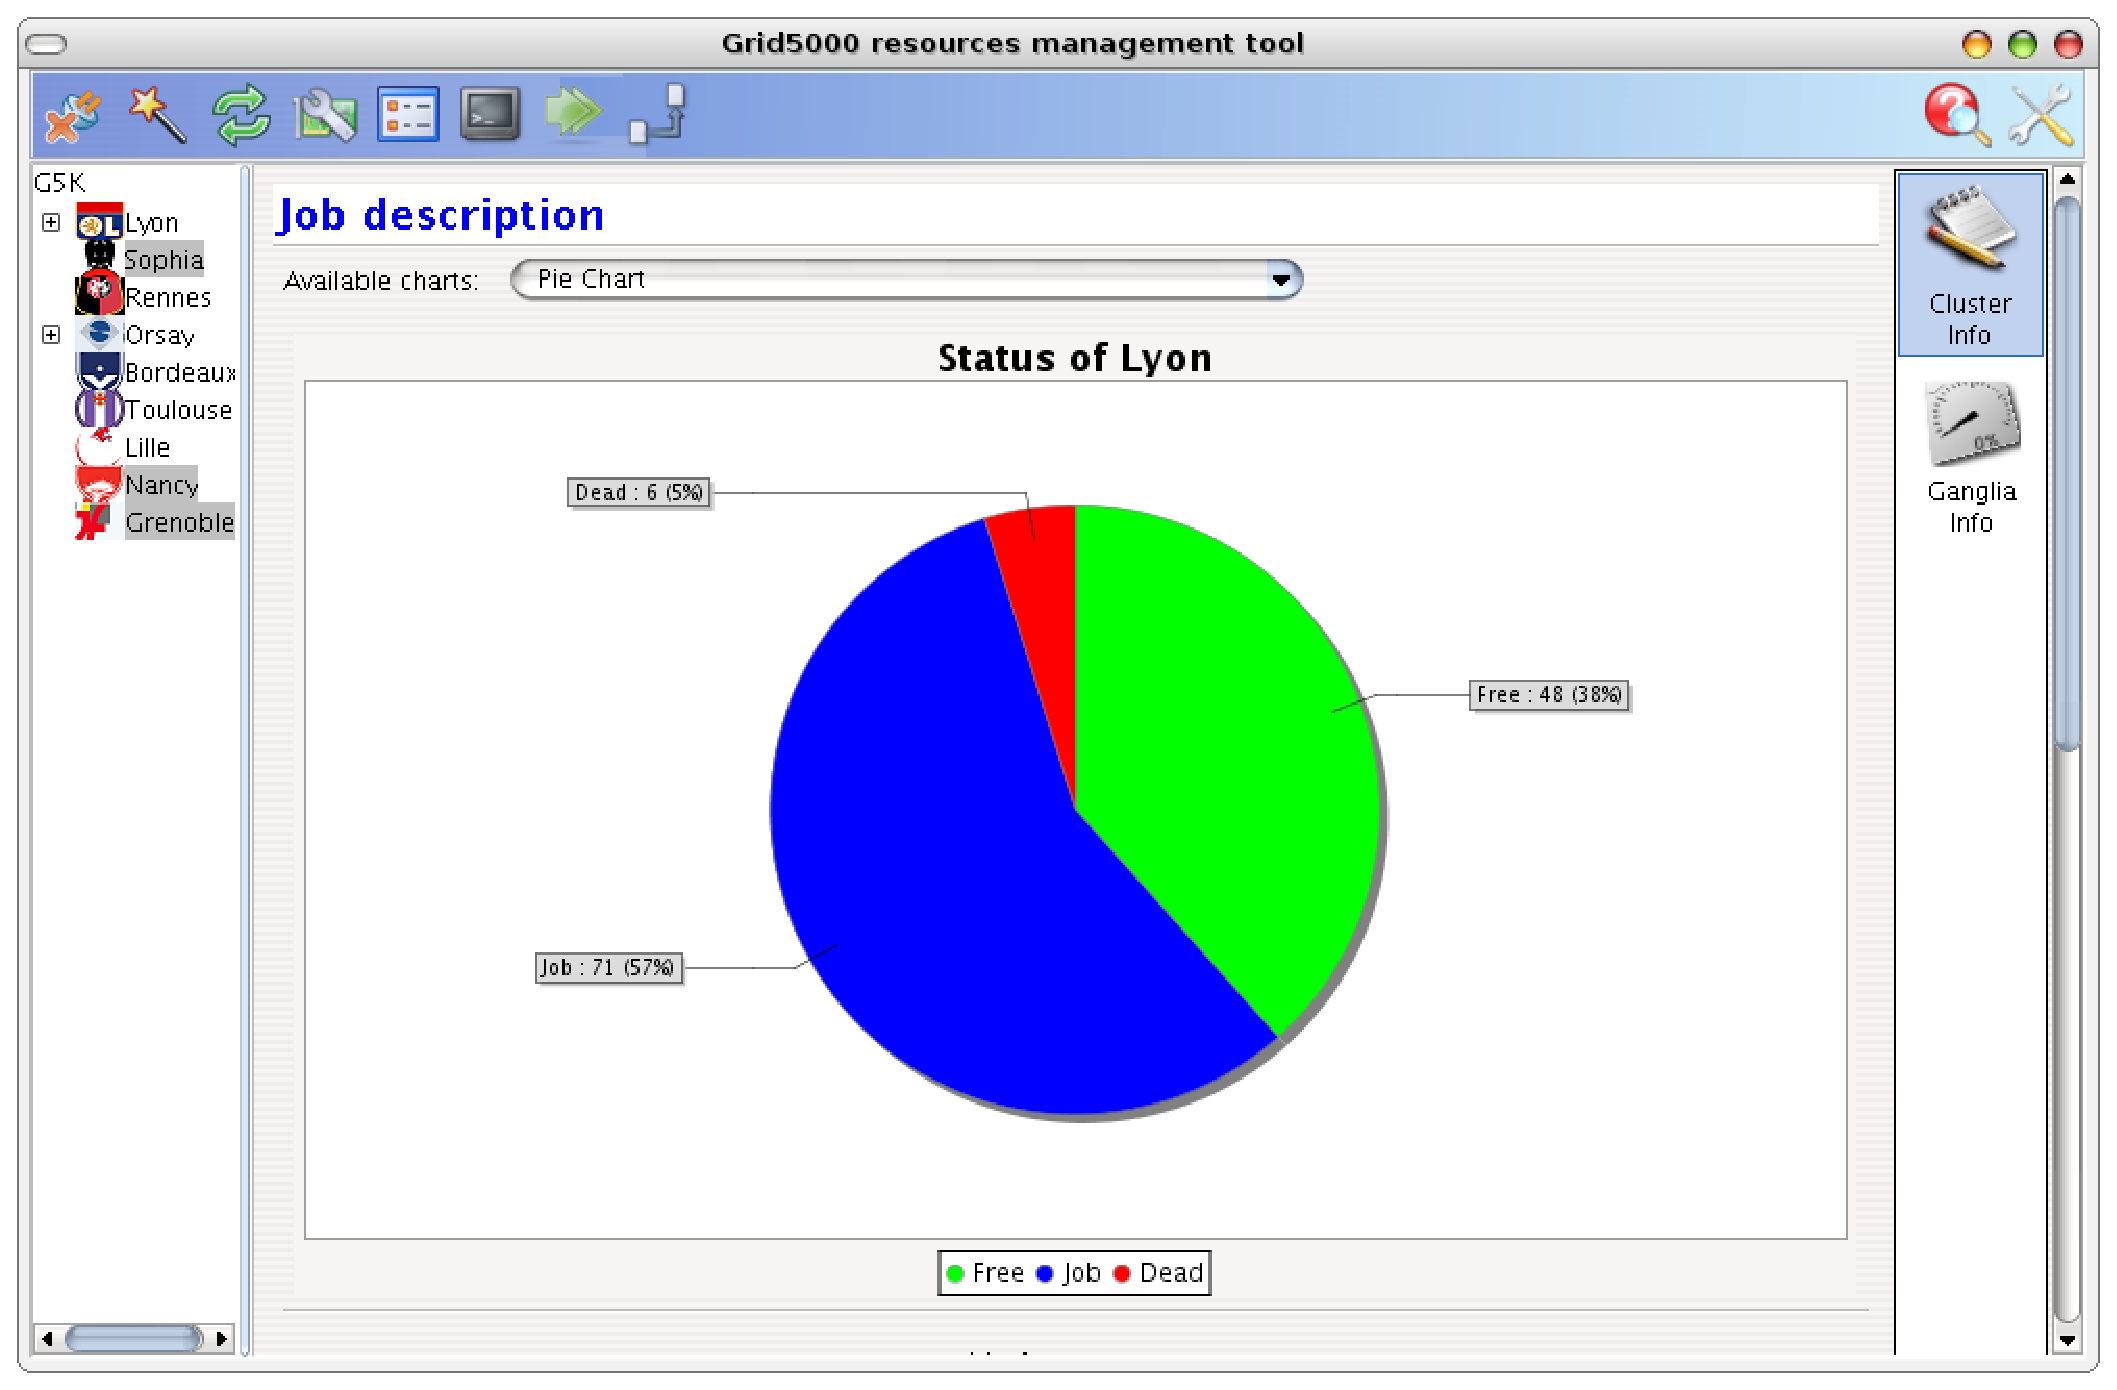
\includegraphics[width=0.5\linewidth]{figures/GRUDU_interface3.eps} &
  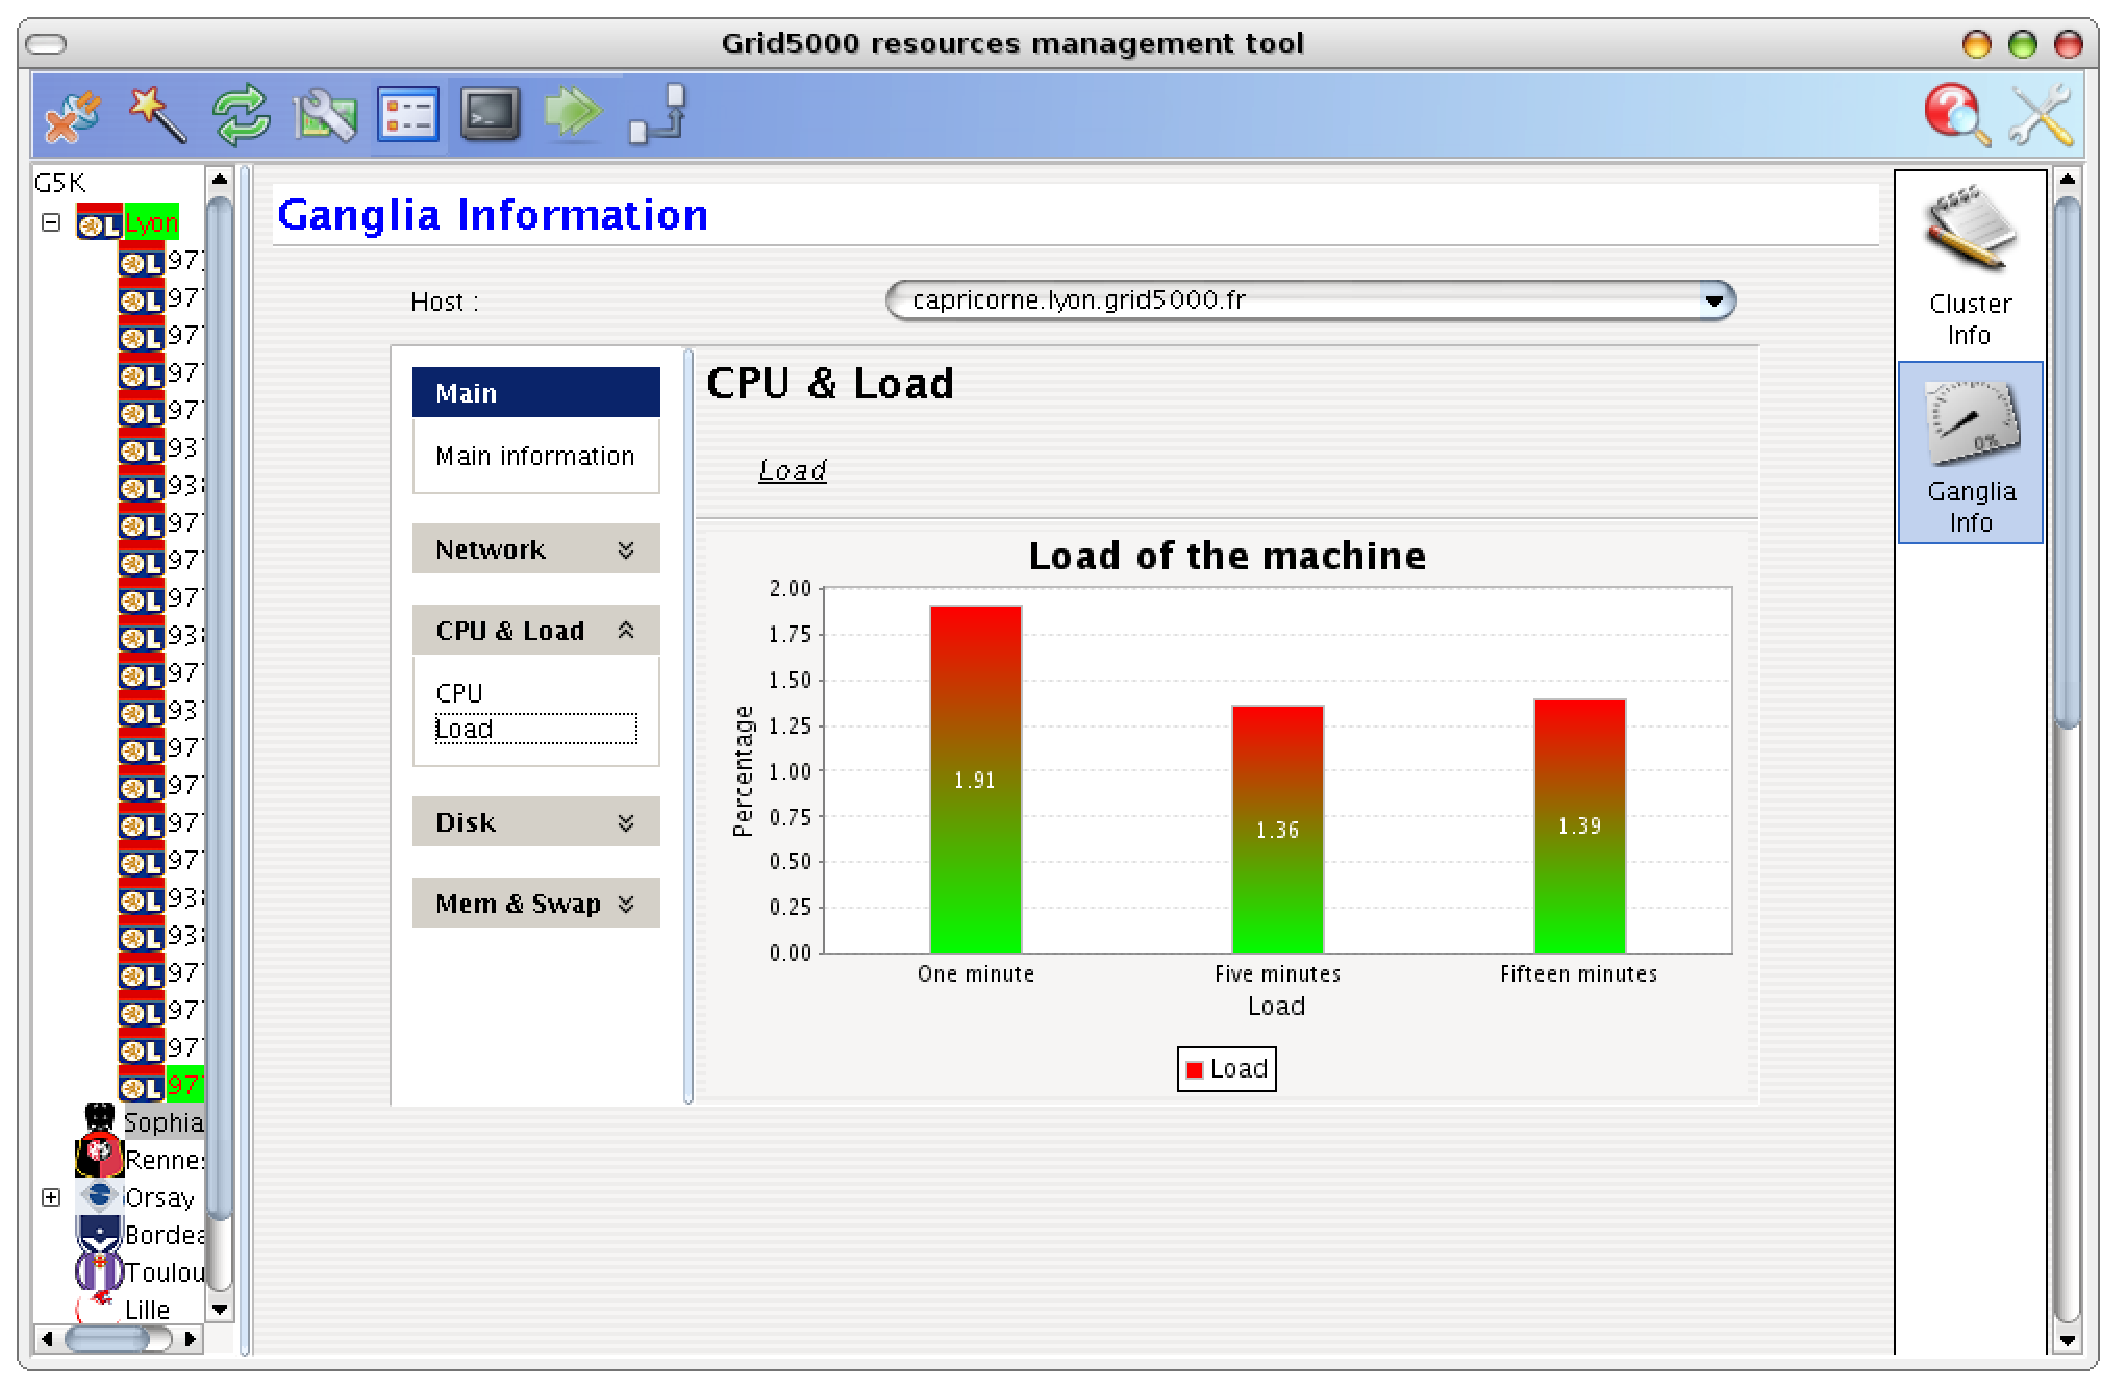
\includegraphics[width=0.5\linewidth]{figures/GRUDU_interface3_ganglia.eps}
  \end{tabular}
	\caption{Site view}
	\label{fig:GRUDU_view_site}
  \end{figure}
  \item  The third view in figure \ref{fig:GRUDU_view_job} corresponds to the
  job view. Here you can see the different information of the job such as the
  nodes of the reservation, the job state, the walltime, etc \ldots
  
  If you selected the Ganglia plugin at the installation step, you also have a
  button bar on the right hand side of the frame that will be populated with a
  Ganglia history information button allowing you to get an history on the
  low-level information concerning the nodes of your reservation. \begin{figure}[H]
  \centering
  \begin{tabular}{cc}
  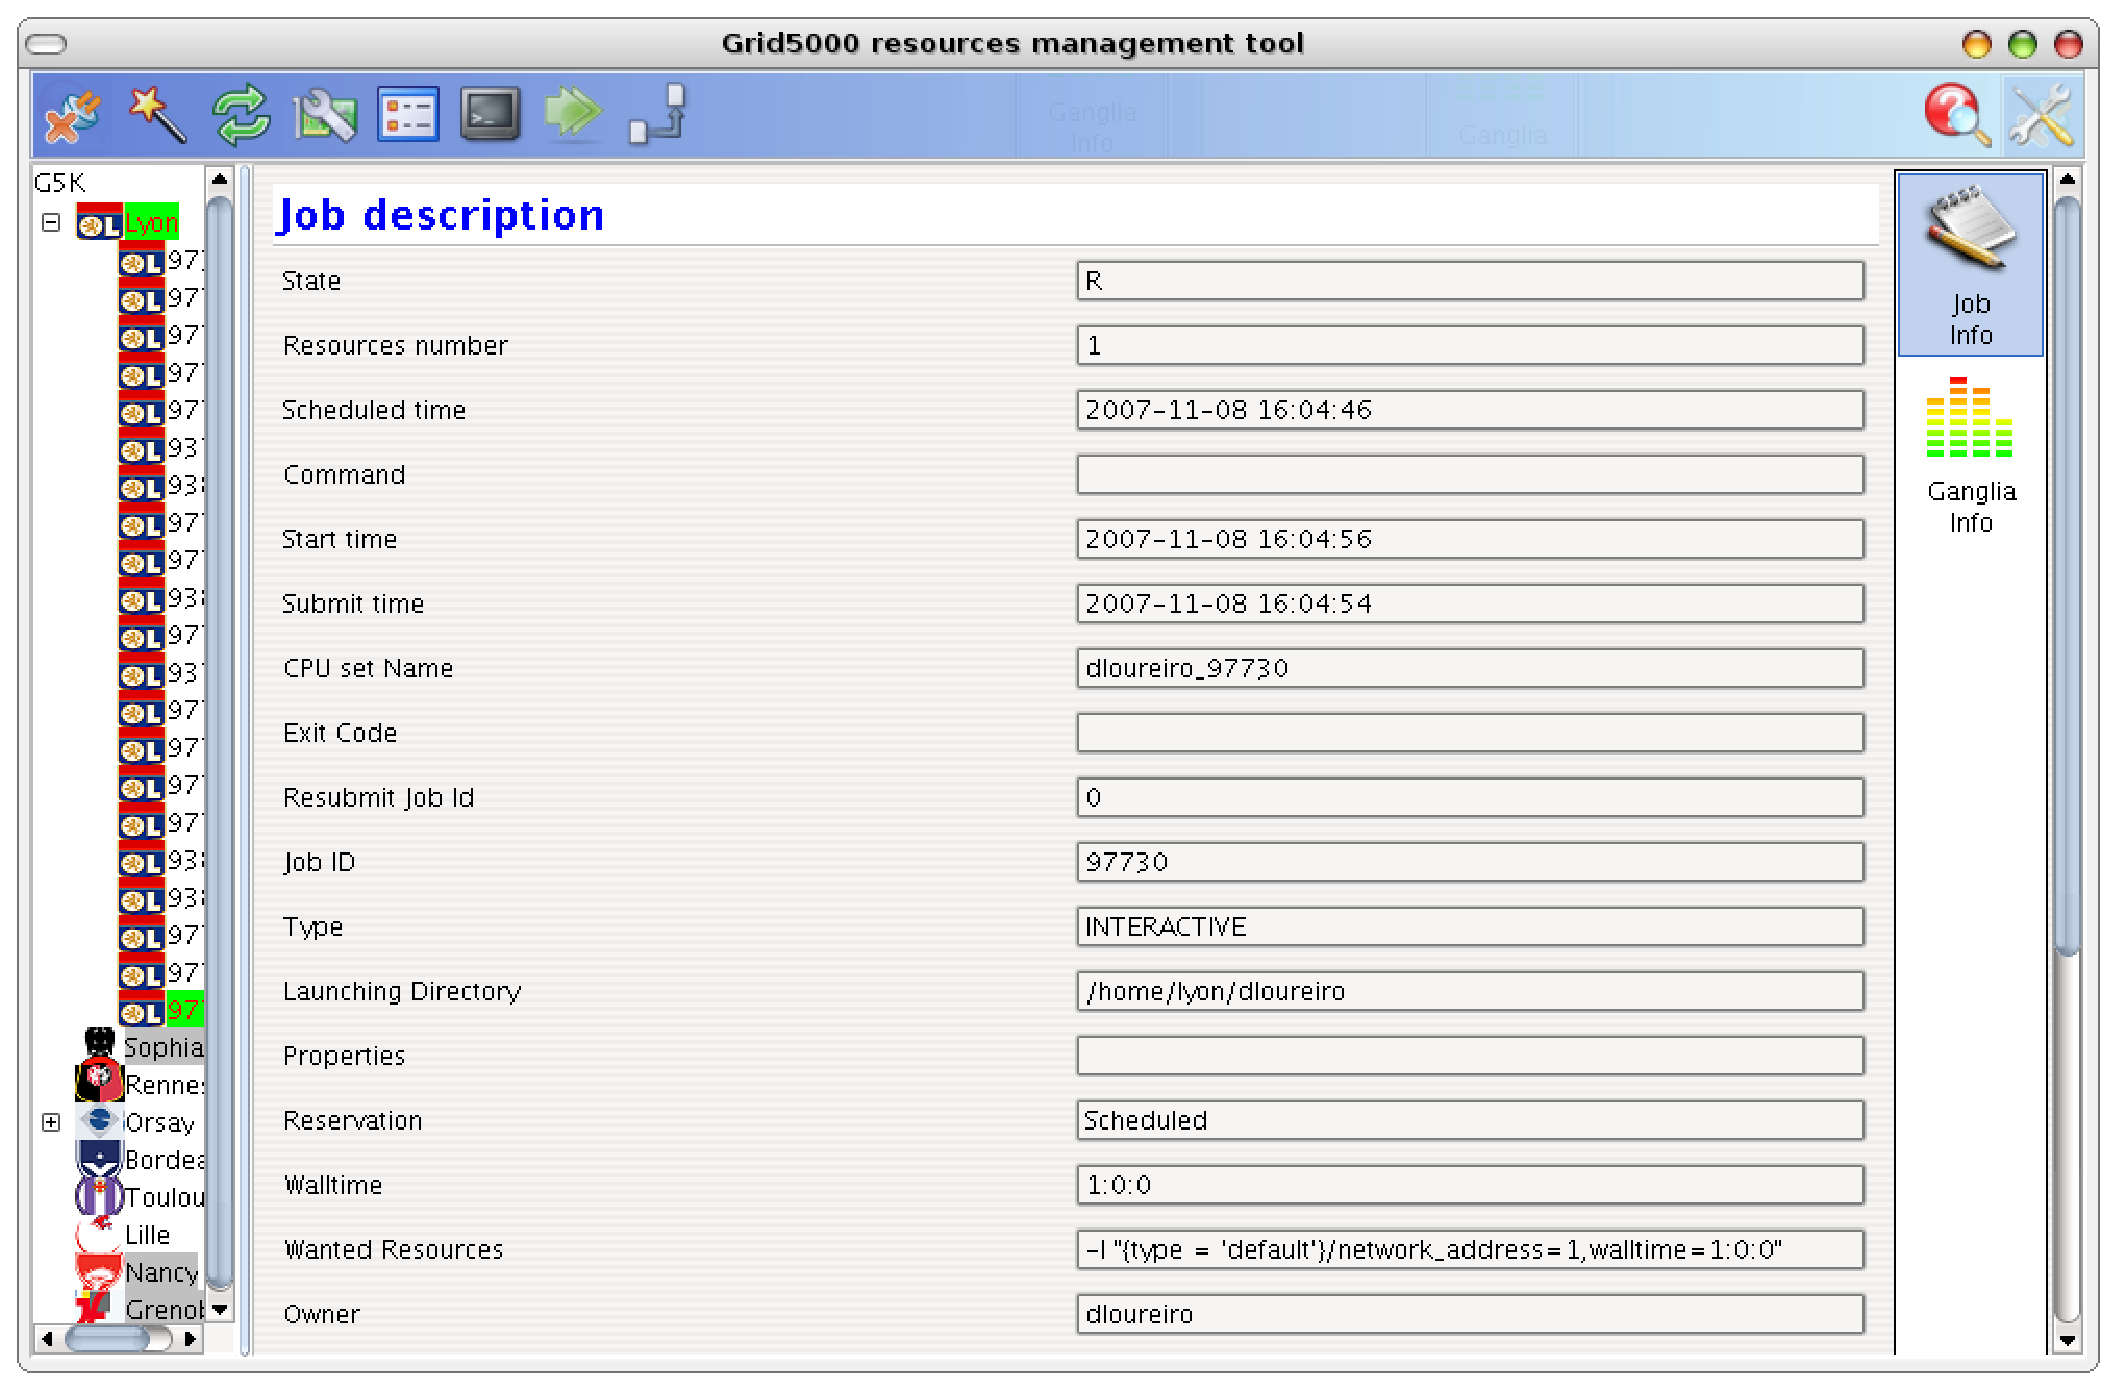
\includegraphics[width=0.5\linewidth]{figures/GRUDU_interface4.eps} &
  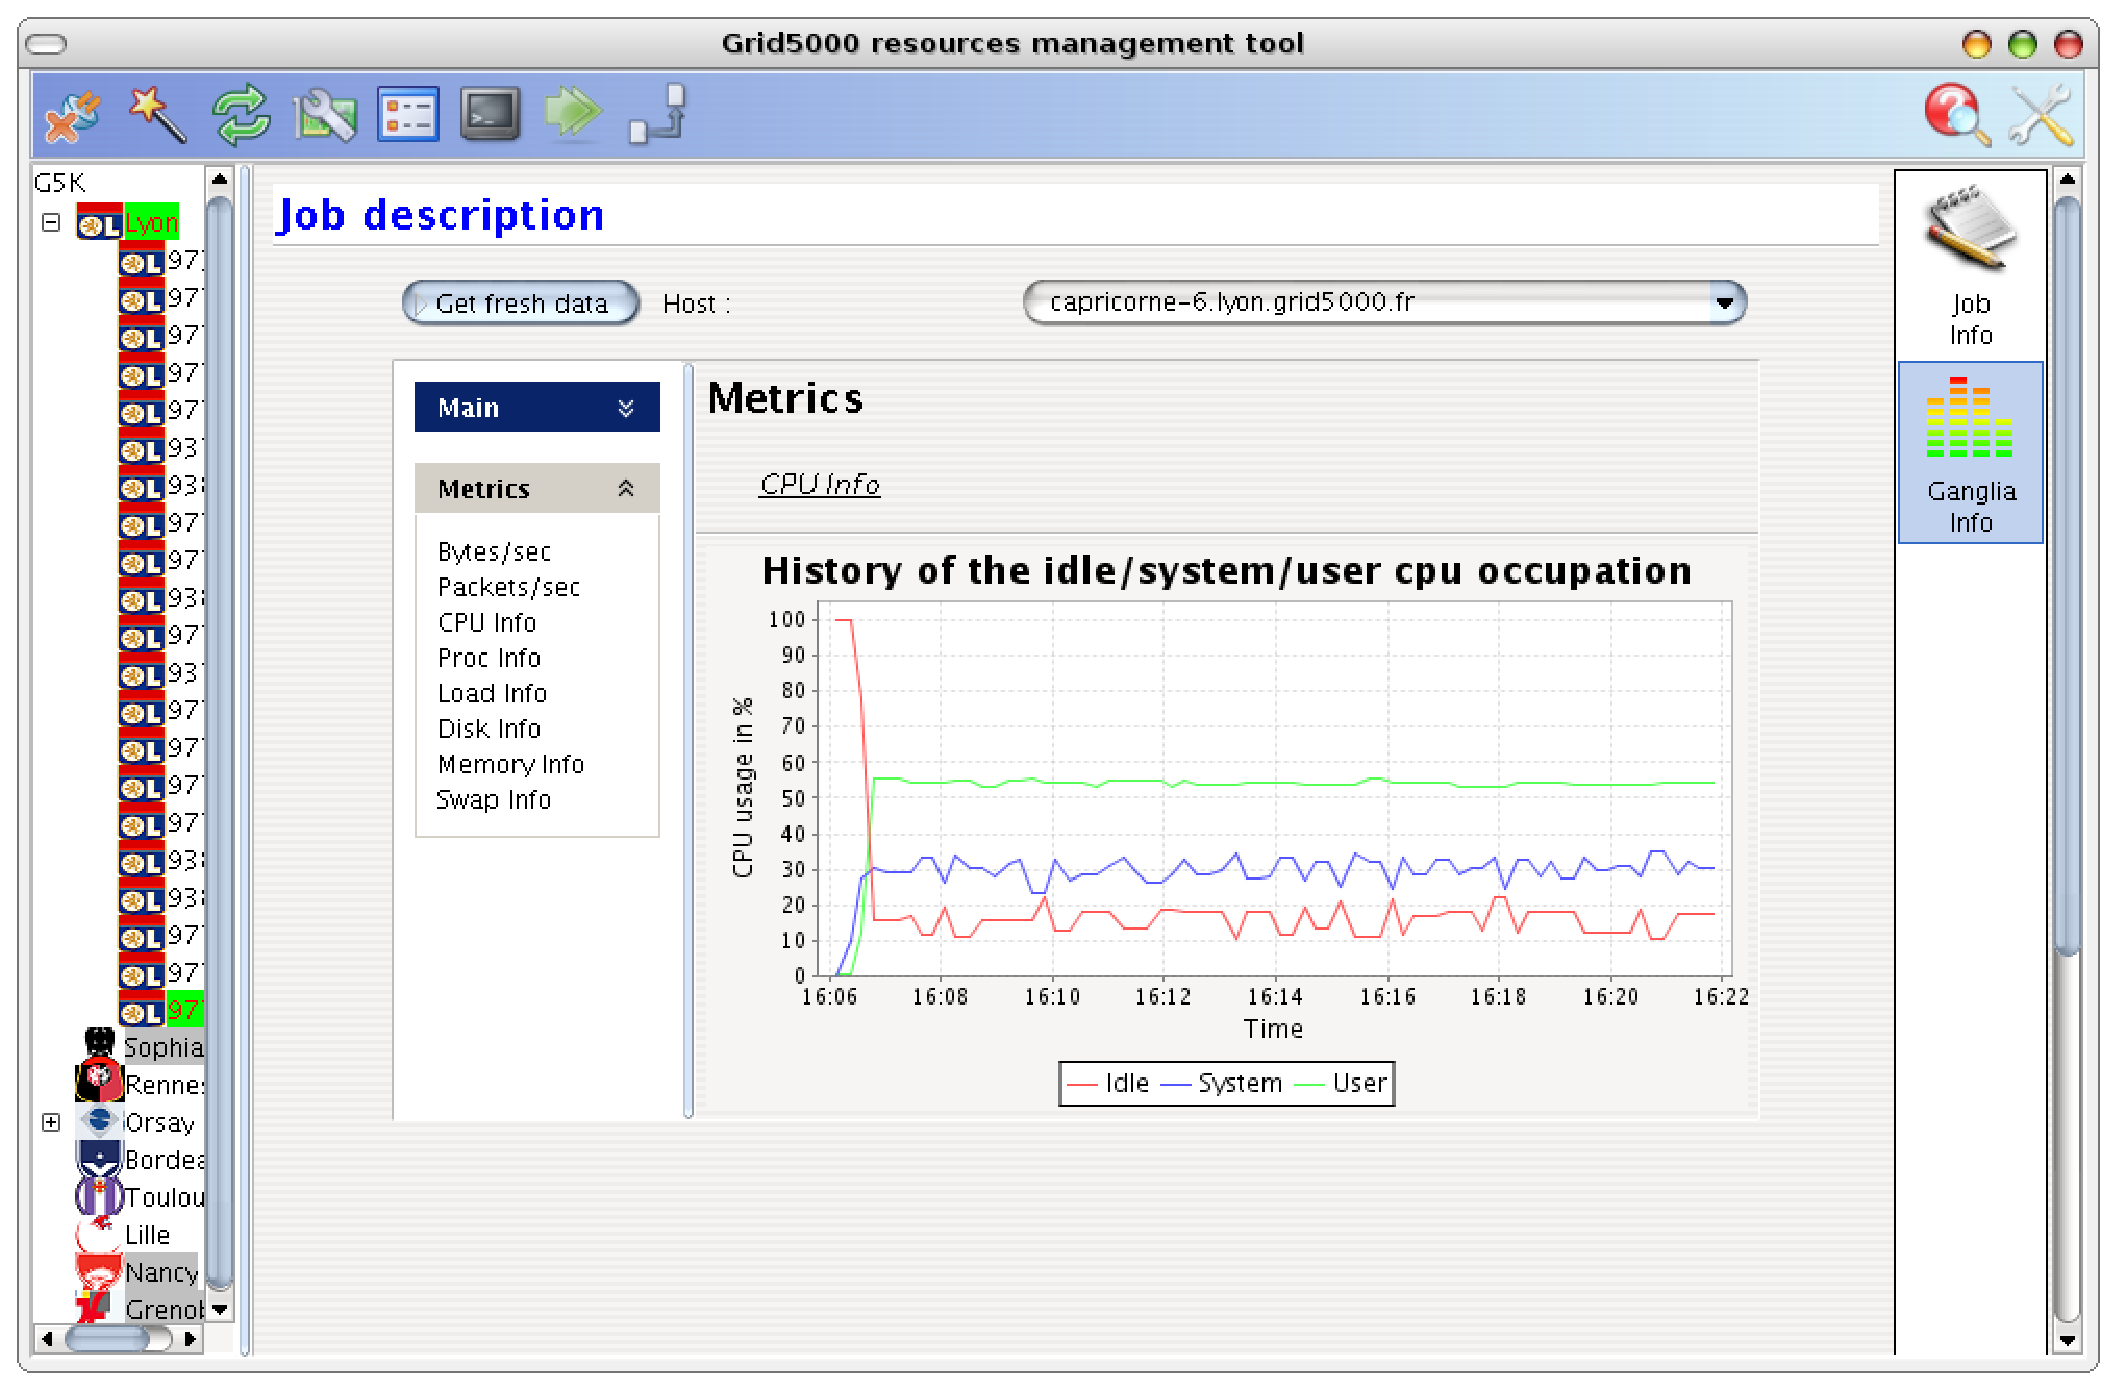
\includegraphics[width=0.5\linewidth]{figures/GRUDU_interface4_ganglia.eps}
  \end{tabular}
	\caption{Job view}
	\label{fig:GRUDU_view_job}
  \end{figure}
\end{itemize}

%******************************************%